\documentclass[12pt]{article}

% ---- Packages ----
\usepackage[margin=1in]{geometry}
\usepackage{amsmath, amssymb, amsthm}
\usepackage{booktabs}
\usepackage{array}
\usepackage{hyperref}
\usepackage{natbib}
\usepackage{graphicx}
\graphicspath{{output/figures/paper/}}
\usepackage{caption}
\usepackage{subcaption}
\usepackage{setspace}
\usepackage{microtype}
\usepackage{xcolor}
\usepackage{titlesec}

% Section fonts: slightly larger than body text, bold; subsections same size, bold
\titleformat{\section}{\large\bfseries}{\thesection.}{0.5em}{}
\titleformat{\subsection}{\normalsize\bfseries}{\thesubsection}{0.5em}{}
\titleformat{\subsubsection}{\normalsize\itshape}{\thesubsubsection}{0.5em}{}
\titlespacing*{\section}{0pt}{1.5ex plus 0.5ex minus 0.2ex}{0.8ex plus 0.1ex}
\titlespacing*{\subsection}{0pt}{1.2ex plus 0.4ex minus 0.2ex}{0.5ex plus 0.1ex}

% \doublespacing  % Uncomment for journal submission requiring double-spaced manuscripts

\hypersetup{
  colorlinks=true,
  linkcolor=blue,
  citecolor=blue,
  urlcolor=blue
}

% ---- Title ----
\title{Double Trouble:\\
Diagnostic Observability in Double Machine Learning Under Weak Overlap}

\author{Acey Vogelstein \and Vy Mai}
\date{April 30, 2026}

\begin{document}

\maketitle

% ---- Abstract ----
\begin{abstract}
Double Machine Learning (DML) provides valid inference for treatment effects by using cross-fitted machine learning models to partial out confounders. However, when the overlap assumption is weak, DML confidence intervals (CIs) can have drastically lower coverage than their nominal level, with no built-in warning. We investigate whether computable diagnostics can detect unreliable DML inference, and find that the answer depends critically on the choice of DML framework (Partially Linear Regression versus Interactive Regression Model). Using semi-synthetic simulations grounded in Infant Health and Development Program (IHDP) covariates (25,000+ estimations), we establish three findings. First, the natural propensity-side diagnostic $R_D = \mathrm{Var}(\tilde{D})/\mathrm{Var}(D)$ is robust to structural propensity misspecification under correct functional form, but blind to outcome model quality. Second, the natural outcome-side diagnostic $R_Y$ (cross-fitted outcome $R^2$) fails under PLR because PLR's outcome model conflates the outcome function with treatment predictability, causing $R_Y$ to move anti-conservatively as overlap weakens. Third, switching to IRM removes this contamination: global treated- and control-arm-specific $R^2$ provides reliable diagnostic signal, and restricting $R^2$ to the extrapolation region (opposite-treatment territory) provides a further improvement when the failure mode is concentrated. The raw diagnostic gap between IRM and PLR, measured by area under the ROC curve (AUC) for predicting CI coverage failure (0.822 vs.\ 0.564), is substantially a learner-composition artifact: the AUC classifier exploits PLR's contaminated $R_Y$ in reverse, which a practitioner interpreting $R_Y$ in the natural direction cannot do. The principal benefit of IRM is therefore structural: it enforces classifiers for propensity by design and eliminates the contamination channel. External validation on LaLonde covariates confirms the core IRM findings but shows the local $R^2$ improvement does not generalize when too few units fall in the extrapolation region. These findings identify a previously underappreciated tradeoff: orthogonalization improves estimation robustness but degrades diagnostic observability.
\end{abstract}

% ===========================================================
% SECTION 1: MOTIVATION
% ===========================================================
\section{Motivation}

Double Machine Learning \citep{Chernozhukov2018} has become a standard tool for estimating average treatment effects from observational data. DML uses machine learning to estimate nuisance functions (the conditional expectation of the outcome and the propensity score) and then constructs a debiased estimator through orthogonalization and cross-fitting. The method provides $\sqrt{n}$-consistent, asymptotically normal estimates even when the nuisance models converge slowly, a powerful theoretical guarantee. However, these guarantees depend on the overlap assumption: every unit must have a non-trivial probability of receiving either treatment. When overlap is weak, meaning when propensity scores approach 0 or 1 for many units, the theoretical guarantees degrade and finite-sample performance can be poor. Nominal 95\% confidence intervals can have actual coverage as low as 24\% in our simulations (Figure~\ref{fig:coverage_collapse}), yet the standard DML output gives no indication of failure.

\begin{figure}[htbp]
  \centering
  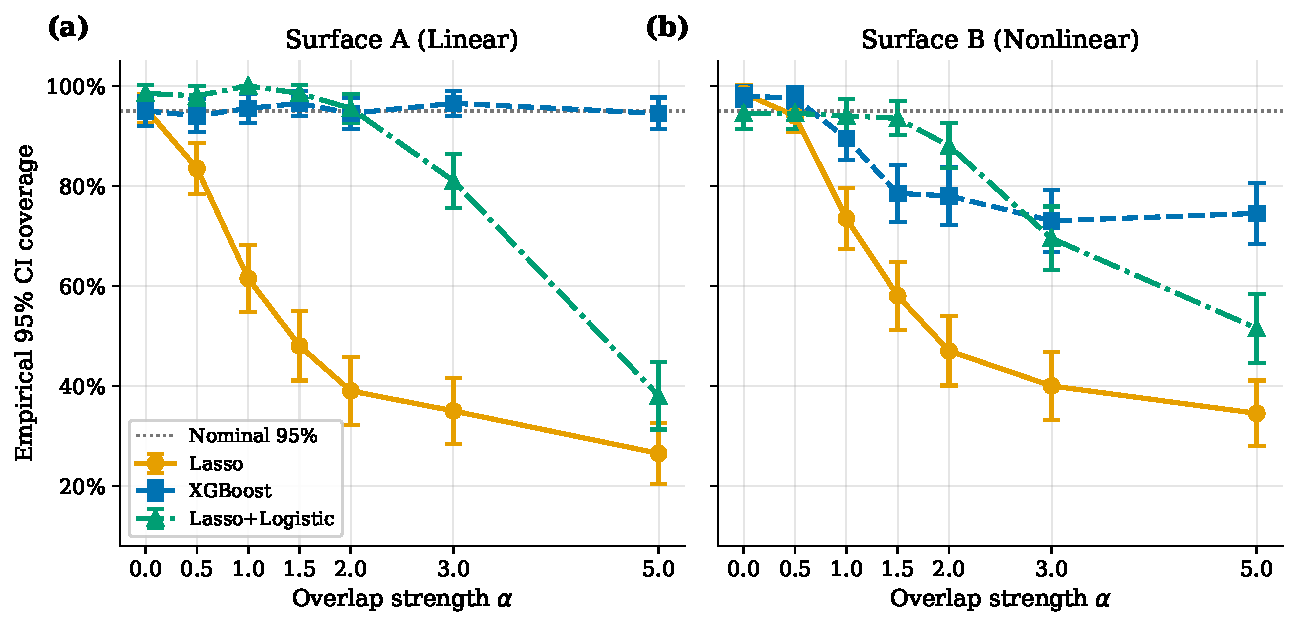
\includegraphics[width=\textwidth]{fig1_coverage_vs_overlap.pdf}
  \caption{Coverage collapse under weak overlap (PLR, structural DGP). Each panel shows empirical 95\% CI coverage as a function of overlap strength $\alpha$ for Lasso, XGBoost, and Lasso+Logistic. Left: linear surface. Right: nonlinear surface. Dashed horizontal line at 95\% indicates nominal coverage.}
  \label{fig:coverage_collapse}
\end{figure}

This raises a practical question: can practitioners detect when their DML estimates are unreliable? The existing literature on DML \citep{Chernozhukov2018, Knaus2022} focuses on estimation consistency and asymptotic normality, establishing \emph{when} DML works, but not on what practitioners can observe about whether the required conditions hold in their data. The overlap literature offers several diagnostics: propensity score trimming rules \citep{Crump2009}, effective sample size from IPW weighting, propensity score distribution checks, and condition number diagnostics \citep{Chernozhukov2025}. But these all address the propensity side of the problem in isolation. Standard outcome model metrics (cross-validated $R^2$, MSE) are available as general-purpose tools, but their informativeness about causal estimation quality under weak overlap has not been studied, and as we show, they can be structurally misleading. We bridge this gap by studying \emph{diagnostic observability} within DML itself: asking not just whether DML fails under weak overlap, but whether the failure is detectable from quantities already produced by the DML pipeline.

We focus on DML for two reasons. First, it is increasingly used in applied economics, policy evaluation, and biostatistics, making its practical failure modes consequential. Second, its two main frameworks, Partially Linear Regression (PLR) and the Interactive Regression Model (IRM), differ structurally in what diagnostics they expose, offering a clean within-method comparison that isolates the effect of framework choice on observability rather than on estimation quality. DML is distinct from simpler propensity-score or regression-adjustment methods \citep{Rosenbaum1983} precisely because its orthogonalization step is designed to make the target estimate robust to nuisance model errors. Yet that same property creates a diagnostic blind spot: the residualization that insulates the treatment-effect estimate from nuisance errors also makes it harder to gauge how reliable those nuisance estimates are. This tension between estimation robustness and diagnostic observability is our central research question, and to the best of our knowledge it has not been directly examined in the simulation literature on DML.

% ===========================================================
% SECTION 2: DML METHODS
% ===========================================================
\section{DML Methods}

DML is used when researchers want to estimate causal effects from observational data with potentially complex, high-dimensional confounding. It is preferred over simpler methods such as OLS or propensity score matching when the relationship between covariates and outcome or treatment is expected to be nonlinear, or when the covariate space is large enough that parametric specifications are likely to be misspecified. DML is increasingly the default choice in applied economics and policy evaluation when researchers want the flexibility of machine learning models without sacrificing valid asymptotic inference for the treatment effect \citep{Knaus2022}.

\subsection{How does DML work?}

DML proceeds in three steps:

\begin{enumerate}
  \item \textbf{Nuisance estimation with cross-fitting.} Split the data into $K$ folds. For each fold $k$, train ML models on the remaining $K-1$ folds to estimate the nuisance functions, then generate out-of-fold predictions for fold $k$. This yields cross-fitted predictions $\hat{g}(X_i)$ and $\hat{m}(X_i)$ for every unit $i$ without any unit appearing in its own training set.

  \item \textbf{Residualization.} Compute orthogonalized residuals:
  \[
    \tilde{Y}_i = Y_i - \hat{g}(X_i), \qquad \tilde{D}_i = D_i - \hat{m}(X_i).
  \]
  These residuals remove the linear influence of the confounders from both the outcome and the treatment assignment.

  \item \textbf{Target parameter estimation.} Estimate $\tau$ by regressing $\tilde{Y}$ on $\tilde{D}$ (in PLR) or by applying a doubly-robust influence-function score (in IRM). Standard errors and confidence intervals follow from the empirical influence function of the resulting estimator.
\end{enumerate}

\subsection{How do PLR and IRM differ?}

\textbf{PLR} estimates a single outcome nuisance function $\hat{g}(X) \approx \mathbb{E}[Y \mid X]$. A critical structural property of PLR is that
\[
  \mathbb{E}[Y \mid X] = g_0(X) + \tau \cdot m_0(X),
\]
so the outcome model's prediction target conflates the baseline outcome function $g_0$ with the propensity score $m_0$, scaled by $\tau$. This conflation has important consequences for the informativeness of outcome-model diagnostics, which we analyze in Section~\ref{sec:results}.

\noindent\textbf{IRM} estimates arm-specific outcome functions separately:
\[
  \hat{g}_0(X) \approx \mathbb{E}[Y \mid X, D=0], \qquad \hat{g}_1(X) \approx \mathbb{E}[Y \mid X, D=1].
\]
These targets do not contain the $\tau \cdot m_0(X)$ term. IRM then applies a doubly-robust score that combines both outcome models with the propensity model, providing protection against misspecification of either nuisance component. This structural difference (estimating $\mathbb{E}[Y \mid X, D=d]$ rather than $\mathbb{E}[Y \mid X]$) is precisely what enables clean outcome-side diagnostics under IRM.

\subsection{Comparison to Traditional Methods}

Compared to OLS regression adjustment, DML allows any ML model for confounding rather than requiring correct parametric specification of $\mathbb{E}[Y \mid X, D]$. Compared to inverse probability weighting (IPW), DML does not require a correctly specified propensity model alone; rate double robustness means that errors in one nuisance model can be compensated by sufficient quality in the other. Compared to augmented IPW (AIPW) estimated parametrically, DML extends double robustness to the nonparametric ML setting through cross-fitting, which prevents the regularization bias that would otherwise inflate variance when ML models are fit on the full sample.

% ===========================================================
% SECTION 3: ASSUMPTIONS
% ===========================================================
\section{Assumptions}

DML relies on three structural identification assumptions and additional regularity conditions for valid inference.

\medskip
\noindent\textbf{Assumption 1: Ignorability (Unconfoundedness).} Conditional on observed covariates $X$, treatment assignment $D$ is independent of potential outcomes:
\[
  \bigl(Y(0),\, Y(1)\bigr) \;\perp\; D \;\Big|\; X.
\]
This requires that all confounders are observed and included in the covariate set. In our simulations, ignorability holds by construction: we generate treatment from known functions of the covariates and outcomes from separate known functions, so no unmeasured confounding is present.

\medskip
\noindent\textbf{Assumption 2: Stable Unit Treatment Value Assumption (SUTVA).} Each unit's outcome depends only on its own treatment status, not on the treatment of other units. There is no interference between units. Our simulations satisfy SUTVA by generating each unit's outcomes independently.

\medskip
\noindent\textbf{Assumption 3: Overlap (Positivity).} For all values of the covariate vector $X$ in the population,
\[
  0 \;<\; P(D = 1 \mid X) \;<\; 1.
\]
Every unit must have a non-zero probability of being in either treatment group. This is the assumption we deliberately vary. At overlap strength $\alpha = 0$, treatment is random and overlap is perfect. As $\alpha$ increases, propensity scores approach 0 or 1 for some covariate subgroups, progressively violating overlap in a controlled manner. We clip propensities at $[0.001, 0.999]$ to maintain strict positivity, but near-boundary values are sufficient to degrade finite-sample performance substantially.

\medskip
\noindent\textbf{Regularity conditions for DML.} Beyond identification, DML requires that the nuisance estimators, the outcome model $\hat{g}$ and propensity model $\hat{m}$, converge at sufficiently fast rates. Specifically, the product of their $L_2$ convergence rates must be $o(n^{-1/2})$. This ``rate double robustness'' condition is what allows DML to achieve $\sqrt{n}$-consistency even with nonparametric nuisance models. In finite samples, the quality of the nuisance models matters considerably: poor outcome models or poor propensity models can inflate bias and degrade coverage even when all three identification assumptions hold.

\medskip
\noindent\textbf{Parametric assumptions.} PLR imposes a partially linear structure:
\[
  Y = \tau D + g_0(X) + \varepsilon,
\]
where the treatment effect $\tau$ is constant (homogeneous) across units. IRM relaxes this by allowing heterogeneous treatment effects through arm-specific outcome models $\mathbb{E}[Y \mid X, D=d] = g_d(X)$, $d \in \{0,1\}$. Both frameworks are nonparametric in the nuisance functions ($g_0$, $g_d$, and $m_0$ are estimated with machine learning) but parametric in the treatment effect representation (a single scalar $\tau$ in PLR; a weighted average in IRM). We use 5-fold cross-fitting throughout to prevent overfitting bias from the nuisance estimation stage, consistent with the theoretical requirements of \citet{Chernozhukov2018}.

% ===========================================================
% SECTION 4: STUDY DESIGN
% ===========================================================
\section{Study Design}

\subsection{Target Estimand}

The target estimand is the \textbf{Average Treatment Effect (ATE)}:
\[
  \tau \;=\; \mathbb{E}\!\left[Y(1) - Y(0)\right].
\]
In words: the average difference in potential outcomes if the entire population were assigned to treatment versus if the entire population were assigned to control. This represents the expected gain from universally adopting the treatment, averaging over all individuals in the population regardless of their observed treatment status.

We choose ATE rather than the Average Treatment Effect on the Treated (ATT) or on the Controls (ATC) for two reasons. First, ATE is the default estimand for both PLR and IRM as implemented in the \texttt{doubleml} package, ensuring that our simulation targets are aligned with the estimator's inferential machinery. Second, ATE is the most demanding estimand with respect to overlap: computing ATE requires outcome model extrapolation for \emph{both} arms. The control outcome model $g_0$ must generalize to treated units, and the treated outcome model $g_1$ must generalize to control units. By contrast, ATT only requires extrapolation from the control model into the treated population. This makes ATE the natural choice for studying diagnostic observability under weak overlap, since the overlap violation affects the estimand from both directions. In our simulation, $\tau = 4.0$ by construction across all outcome surfaces and all replications.

\subsection{Simulation Design}

We are primarily concerned with the \textbf{overlap assumption} and its interaction with \textbf{outcome model quality}. Specifically, we explore four dimensions:

\begin{enumerate}
  \item \textbf{Overlap violation severity.} As propensity scores become more extreme (closer to 0 or 1), DML's finite-sample performance degrades. We vary overlap strength $\alpha$ from 0 (perfect overlap, random treatment) to 5 (severe violation), providing a continuous spectrum of the overlap assumption's satisfaction.

  \item \textbf{Outcome model complexity.} A linear outcome surface is easy for all learners; a nonlinear surface challenges linear learners such as Lasso. This interacts with overlap: when overlap is weak, the outcome model must extrapolate in covariate regions with few training observations, and model quality in those regions determines whether causal inference succeeds.

  \item \textbf{Propensity model specification.} The propensity model can be correctly specified (XGBoost, which captures a race--birthweight interaction in the true DGP) or misspecified (Lasso, which cannot capture interactions). This affects both estimation quality and the reliability of the propensity diagnostic $R_D$.

  \item \textbf{DML framework choice (PLR vs.\ IRM).} PLR and IRM differ structurally in what diagnostics they expose. We evaluate whether switching frameworks improves diagnostic observability: the ability to detect, from within the DML output itself, when inference is unreliable.
\end{enumerate}

\noindent\textbf{Base data.} We use covariates from the Infant Health and Development Program (IHDP), a randomized trial of 985 infants with 28 covariates covering birthweight, neonatal health, maternal demographics, and birth circumstances. Our semi-synthetic simulation framework (generating synthetic treatment and outcomes over fixed real covariates to benchmark causal inference under lack of common support) follows the design introduced by \citet{Hill2011} and further developed in \citet{Hill2012}. The covariate matrix is fixed across all replications; treatment assignment and outcomes are generated synthetically.

\medskip
\noindent\textbf{DGP 1: Assumptions satisfied ($\alpha = 0$).} Treatment is assigned randomly with $p = 0.38$ for all units, satisfying the overlap assumption exactly. Both outcome surfaces are generated from \citet{Hill2011} response surfaces with true ATE $= 4.0$. Under this DGP, all learners should achieve nominal 95\% coverage, providing a baseline against which violations can be measured.

\medskip
\noindent\textbf{DGP 2+: Overlap assumption violated ($\alpha \in \{0.5, 1.0, 1.5, 2.0, 3.0, 5.0\}$).} Treatment probability depends on a race $\times$ birthweight interaction through a structural propensity model inspired by \citet{Hill2011}:
\begin{align*}
  \text{Non-white mothers:} &\quad \mathrm{logit}(p) = \text{baseline} + \alpha\,(0.5 - 1.5 \cdot z_{\text{bw}}) \\
  \text{White mothers:} &\quad \mathrm{logit}(p) = \text{baseline} - \alpha
\end{align*}
As $\alpha$ increases from 0, treatment becomes increasingly predictable from race and birthweight. Lasso cannot capture this interaction structure; XGBoost can. Propensities are clipped at $[0.001, 0.999]$ to maintain strict positivity while still creating near-boundary values.

\medskip
\noindent\textbf{Outcome surfaces} (used in both DGPs):

\begin{itemize}
  \item \emph{Surface A (linear):} $Y(0) \sim \mathcal{N}(X\beta,\, 1)$,\; $Y(1) \sim \mathcal{N}(X\beta + 4,\, 1)$. Constant ATE $= 4$. Coefficients $\beta$ are drawn from $\{0, 1, 2, 3, 4\}$ with probabilities $\{0.5, 0.2, 0.15, 0.1, 0.05\}$ and re-drawn each replication to add outcome heterogeneity.

  \item \emph{Surface B (nonlinear):} $Y(0) \sim \mathcal{N}(\exp((X+0.5)\beta),\, 1)$,\; $Y(1) \sim \mathcal{N}((X+0.5)\beta - \omega,\, 1)$. Heterogeneous effects. $\beta$ drawn from $\{0, 0.1, 0.2, 0.3, 0.4\}$ with probabilities $\{0.6, 0.1, 0.1, 0.1, 0.1\}$. The offset $\omega$ is calibrated each replication so the sample ATE $= 4$.
\end{itemize}

\noindent\textbf{Robustness DGPs.} Three additional propensity models provide robustness checks: a logistic model using 4 clinical covariates, a high-dimensional model with 6 covariates plus 3 interactions, and a threshold model based on step functions in birthweight.

\medskip
\noindent\textbf{Monte Carlo design.} The primary PLR simulation grid consists of 7 overlap strengths $\times$ 2 outcome surfaces $\times$ 200 replications per learner configuration, well exceeding the 1,000-iteration minimum per setup. The IRM grid covers 3 overlap strengths $\times$ 2 surfaces $\times$ 4 learners $\times$ 100 replications $= 2{,}400$ estimations. The PLR and IRM grids use different replication counts (200 vs.\ 100); AUC estimates reported in Table~\ref{tab:auc} therefore have different precision for the two frameworks. All within-IRM improvements are tested with paired bootstrap (2,000 replicates); the PLR--IRM gap is not separately bootstrapped. The raw gap (0.24 AUC points on the linear surface) is substantially a learner-composition artifact, as detailed in Section~\ref{sec:results}. Additional runs explore sample size variation ($n \in \{500, 985, 2000\}$) and the propensity isolation experiment (comparing Lasso vs.\ Lasso+Logistic). The total simulation produces over 25,000 DML estimations.

\subsection{Implementation}

We implement both PLR and IRM using the \texttt{doubleml} Python package (v0.10.1) with 5-fold cross-fitting. Five learner configurations are tested:

\begin{table}[h!]
\centering
\caption{Learner configurations}
\label{tab:learners}
\begin{tabular}{lll}
\toprule
\textbf{Configuration} & \textbf{Outcome model} & \textbf{Propensity model} \\
\midrule
Lasso            & LassoCV                & LassoCV (regression) \\
Lasso+Logistic   & LassoCV                & LogisticRegression \\
Ridge            & RidgeCV                & LogisticRegression \\
XGBoost          & XGBRegressor           & XGBClassifier \\
Random Forest    & RandomForestRegressor  & RandomForestClassifier \\
\bottomrule
\end{tabular}
\end{table}

\noindent The Lasso configuration uses linear regression on a binary treatment outcome, which is a functional form mismatch for the propensity model that inflates the propensity diagnostic. Lasso+Logistic corrects this while holding the outcome model constant, enabling a clean isolation experiment. XGBoost uses fixed hyperparameters (\texttt{max\_depth=3}, \texttt{n\_estimators=100}, \texttt{learning\_rate=0.05}, \texttt{subsample=0.8}). Random Forest uses \texttt{n\_estimators=200}, \texttt{max\_depth=5} and serves as an alternative flexible learner to confirm findings are not XGBoost-specific.

\subsection{Candidate Diagnostics}

We propose and evaluate the following computable diagnostics, all of which are natural byproducts of the DML pipeline:

\begin{itemize}
  \item $R_D = \mathrm{Var}(\tilde{D})/\mathrm{Var}(D)$: propensity-side diagnostic measuring the fraction of treatment variation that remains after partialling out covariates. High $R_D$ indicates good overlap; low $R_D$ indicates weak overlap or near-perfect predictability of treatment.

  \item $R_Y$: cross-fitted $R^2$ of the outcome model. Under PLR this measures how well $\hat{g}(X)$ predicts $Y$. Under IRM, we compute arm-specific versions $R_{Y0}$ and $R_{Y1}$.

  \item $R_{Yd,\text{local}}$: $R^2$ restricted to units in the \emph{extrapolation region}, specifically controls with $\hat{m} > 0.5$ and treated with $\hat{m} < 0.5$, measuring outcome fit precisely where the causal inference problem requires out-of-support extrapolation.
\end{itemize}

% ===========================================================
% SECTION 5: SIMULATION RESULTS
% ===========================================================
\section{Results}
\label{sec:results}

\subsection{Bias, RMSE, and Coverage}

Table~\ref{tab:plr_performance} reports bias, RMSE, and 95\% confidence interval coverage for representative PLR estimations under the structural DGP. Figure~\ref{fig:bias_rmse_coverage} displays all three metrics as a function of overlap strength $\alpha$ for three learners across both surfaces, with 95\% CI bands across replications.

\begin{table}[h!]
\centering
\caption{PLR performance under weak overlap (structural DGP, 200 replications per cell). Coverage is the empirical 95\% CI coverage rate; nominal target is 95\%.}
\label{tab:plr_performance}
\begin{tabular}{llrrr}
\toprule
$\alpha$ & Learner & Bias & RMSE & Coverage \\
\midrule
\multicolumn{5}{l}{\textit{Surface A (Linear)}} \\[2pt]
0.0 & Lasso   & $+0.00$ & 0.15 & 94.0\% \\
0.0 & XGBoost & $-0.03$ & 0.10 & 93.5\% \\
2.0 & Lasso   & $-0.43$ & 0.64 & 39.0\% \\
2.0 & XGBoost & $-0.03$ & 0.16 & 94.5\% \\
5.0 & Lasso   & $-0.64$ & 0.88 & 27.0\% \\
5.0 & XGBoost & $-0.11$ & 0.29 & 94.0\% \\
\midrule
\multicolumn{5}{l}{\textit{Surface B (Nonlinear)}} \\[2pt]
0.0 & Lasso   & $-0.01$ & 0.17 & 98.5\% \\
0.0 & XGBoost & $-0.04$ & 0.17 & 96.5\% \\
2.0 & Lasso   & $-0.21$ & 1.13 & 46.0\% \\
2.0 & XGBoost & $-0.27$ & 0.90 & 74.0\% \\
5.0 & Lasso   & $-0.38$ & 1.59 & 33.5\% \\
5.0 & XGBoost & $-0.31$ & 1.29 & 73.5\% \\
\bottomrule
\end{tabular}
\end{table}

At $\alpha = 0$ (assumptions satisfied), both learners achieve near-nominal coverage with minimal bias. As overlap weakens, Lasso's coverage collapses from 94.0\% to 27.0\% on the linear surface, driven by increasing bias ($-0.64$) and RMSE ($0.88$). XGBoost maintains 94.0\% coverage on the linear surface even at $\alpha = 5$ because it successfully models the race--birthweight interaction in the propensity, but degrades to 73.5\% on the nonlinear surface where outcome extrapolation becomes the binding constraint. The key observation is that \textbf{the same overlap violation produces dramatically different outcomes depending on the learner and outcome surface.} This is precisely what motivates the diagnostic question.

One counterintuitive pattern in Table~\ref{tab:plr_performance} deserves attention: Lasso achieves \emph{higher} empirical coverage on the nonlinear surface (33.5\%) than on the linear surface (27.0\%) at $\alpha = 5$, despite the nonlinear surface being harder to fit. This is not a sign that the nonlinear DGP is more forgiving. On the linear surface, Lasso's outcome model is accurate enough to produce tight confidence intervals that \emph{confidently exclude} the true ATE, yielding low coverage. On the nonlinear surface, Lasso's poor outcome fit inflates residual variance, which inflates the standard error and widens the confidence interval; imprecise estimates cover the truth more often by accident. The relationship between outcome model quality and coverage is therefore non-monotonic: a worse model can produce higher empirical coverage when its errors expand the standard error enough to compensate for bias.

\begin{figure}[htbp]
  \centering
  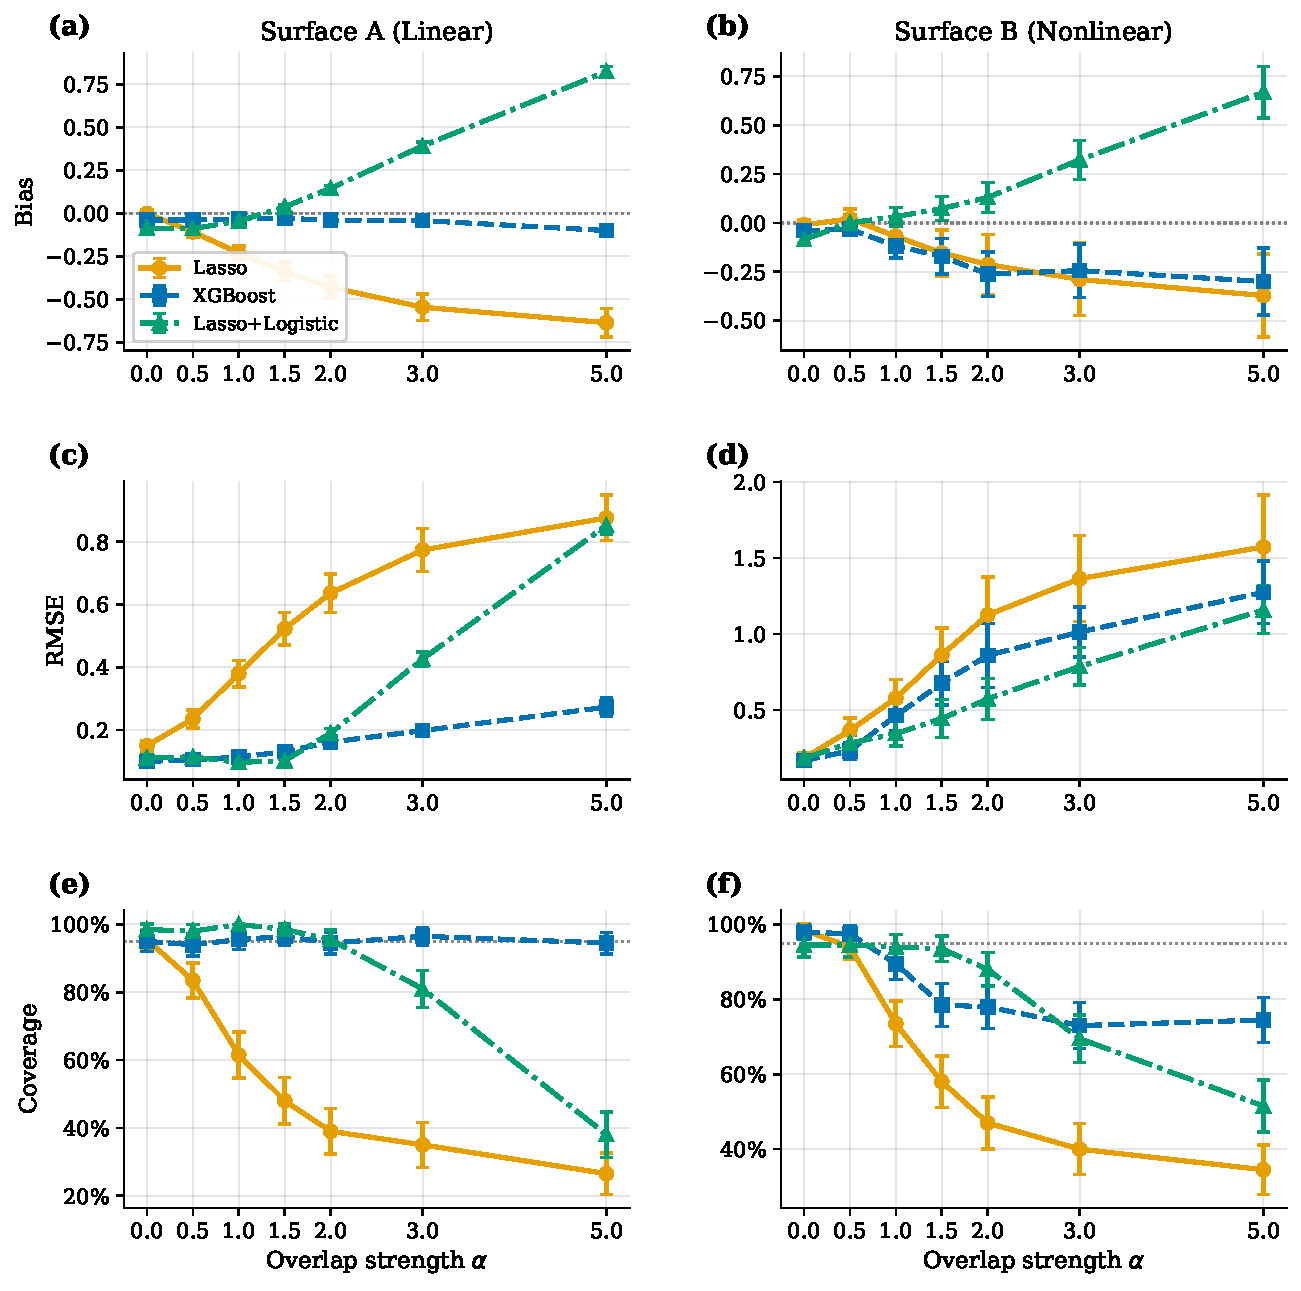
\includegraphics[width=\textwidth]{fig7_bias_rmse_coverage.pdf}
  \caption{Bias, RMSE, and 95\% CI coverage as a function of overlap strength $\alpha$ for three learners (Lasso, XGBoost, Lasso+Logistic) across both outcome surfaces. $3 \times 2$ panel grid with 95\% CI bands across Monte Carlo replications.}
  \label{fig:bias_rmse_coverage}
\end{figure}

\subsection{Propensity-Side Diagnostic: $R_D$}

\noindent\textbf{The inflation identity.} Under propensity misspecification, $R_D$ decomposes as
\[
  R_D \;=\; R_D^* \;+\; \frac{\mathrm{Var}(\delta)}{\mathrm{Var}(D)},
\]
where $R_D^*$ is the oracle diagnostic and $\delta$ represents the misspecification error. Misspecification always inflates $R_D$ upward (anti-conservative). We verify this empirically with decomposition residuals $< 1.59 \times 10^{-5}$.

\noindent\textbf{Behaviour at perfect overlap.} At $\alpha = 0$, treatment is random and the true propensity is constant at $p = 0.38$, so there is no signal for the propensity model to learn. Flexible learners such as XGBoost can slightly overfit in cross-fitting folds, producing out-of-fold predictions that are weakly anti-correlated with the true propensity. This causes $\mathrm{Var}(\tilde{D}) > \mathrm{Var}(D)$ and yields $R_D$ marginally above 1 (observed: 1.04 for XGBoost at $\alpha = 0$). This artefact is a finite-sample property of flexible models with no true signal; it disappears as $\alpha$ increases and the propensity acquires structure to learn.

\noindent\textbf{Robustness to structural misspecification.} At $\alpha = 5$, Lasso using regression on a binary treatment shows $R_D = 0.66$, while XGBoost shows $R_D = 0.15$. This dramatic gap is primarily a functional form error. Switching Lasso's propensity model to logistic regression (Lasso+Logistic) reduces $R_D$ to $0.19$, only $+0.055$ above the oracle $R_D^* = 0.139$. With correct functional form, structural misspecification produces only modest inflation.

\noindent\textbf{Outcome-side blindness.} $R_D$ is necessary but not sufficient for diagnosing DML reliability. At similar $R_D$ values (${\sim}0.15$--$0.22$, under IRM at $\alpha = 5$), coverage varies dramatically:

\begin{table}[h!]
\centering
\caption{Outcome-side blindness: similar $R_D$ values, widely different coverage (IRM, $\alpha = 5$). Variation is driven entirely by outcome model quality, which $R_D$ cannot detect.}
\label{tab:blindness}
\begin{tabular}{lrrr}
\toprule
Learner & $R_D$ & Coverage (Linear) & Coverage (Nonlinear) \\
\midrule
XGBoost          & 0.149 & 70\% & 90\% \\
Ridge            & 0.194 & 62\% & 84\% \\
Lasso+Logistic   & 0.195 & 56\% & 85\% \\
Random Forest    & 0.217 & 29\% & 66\% \\
\bottomrule
\end{tabular}
\end{table}

\noindent The same overlap signal ($R_D$), but coverage ranging from 29\% to 90\% (Figure~\ref{fig:blindness}). This variation is entirely driven by outcome model quality, which $R_D$ is structurally blind to.

\begin{figure}[htbp]
  \centering
  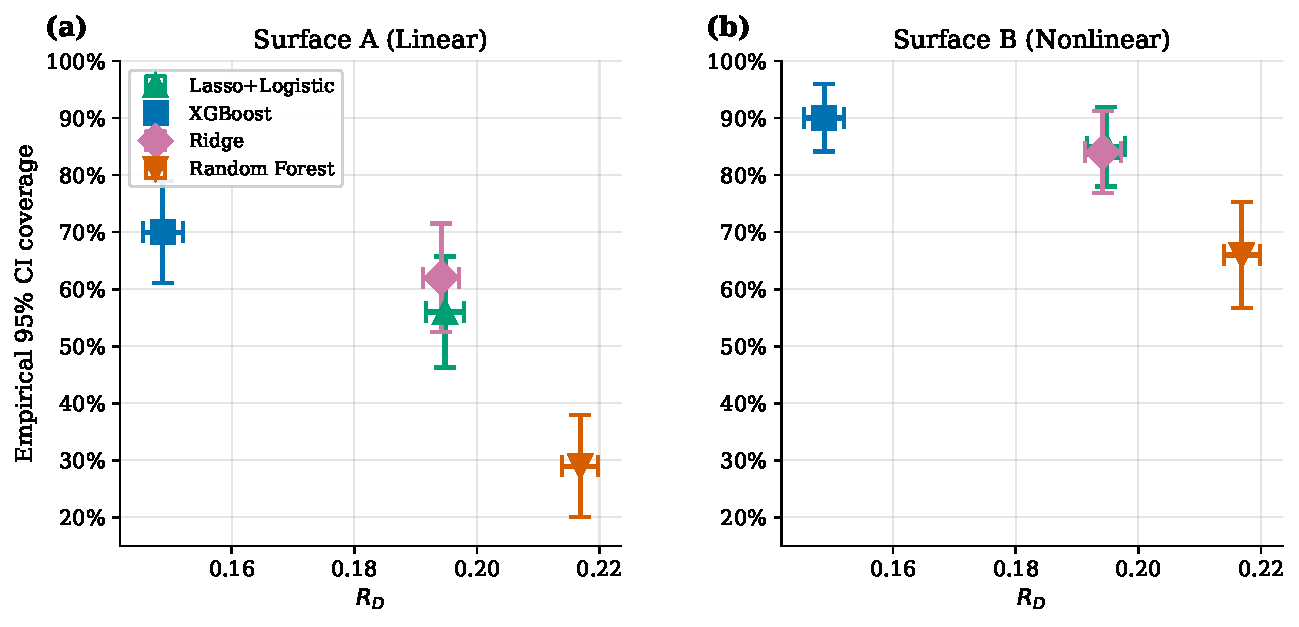
\includegraphics[width=\textwidth]{fig2_outcome_side_blindness.pdf}
  \caption{Outcome-side blindness under IRM at $\alpha = 5$. Learners with similar $R_D$ values show widely different coverage (see Table~\ref{tab:blindness}), demonstrating that the propensity diagnostic alone is insufficient.}
  \label{fig:blindness}
\end{figure}

\subsection{Outcome-Side Diagnostics: PLR Fails, IRM Succeeds}

\noindent\textbf{PLR's $R_Y$ is contaminated.} In PLR, $\hat{g}(X)$ estimates $\mathbb{E}[Y \mid X] = g_0(X) + \tau \cdot m_0(X)$. As overlap weakens, $m_0(X)$ becomes more variable and predictable, so $R_Y$ mechanically rises as the propensity component becomes easier to fit, even as coverage falls. For XGBoost on the nonlinear surface, $R_Y$ increases from 0.357 ($\alpha = 0$, 98.0\% coverage) to 0.723 ($\alpha = 5$, 74.5\% coverage). The diagnostic moves in the wrong direction (Figure~\ref{fig:plr_contamination}).

\begin{figure}[htbp]
  \centering
  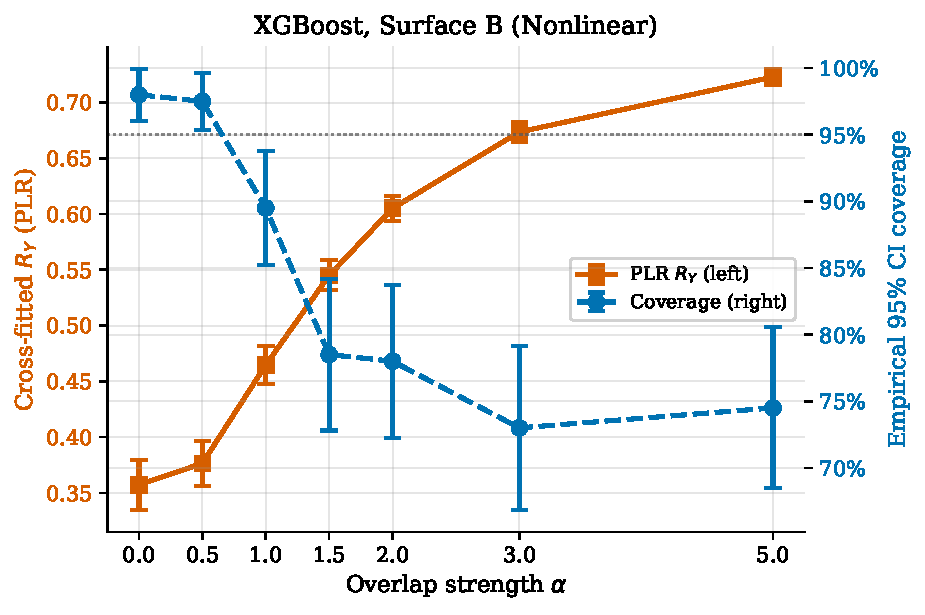
\includegraphics[width=\textwidth]{fig3_plr_contamination.pdf}
  \caption{PLR contamination. Dual-axis plot for XGBoost on the nonlinear surface: as $\alpha$ increases, $R_Y$ rises (left axis) while coverage falls (right axis). The diagnostic moves in the wrong direction.}
  \label{fig:plr_contamination}
\end{figure}

\noindent\textbf{IRM removes the contamination.} IRM estimates $\mathbb{E}[Y \mid X, D=d]$ separately for each arm, so arm-specific $R_{Y0}$ does not contain the treatment predictability channel. XGBoost's $R_{Y0}$ remains stable across overlap levels on the linear surface ($0.843 \to 0.832 \to 0.832$), unlike PLR's $R_Y$ which nearly doubles on the nonlinear surface (Figure~\ref{fig:irm_vs_plr}).

\begin{figure}[htbp]
  \centering
  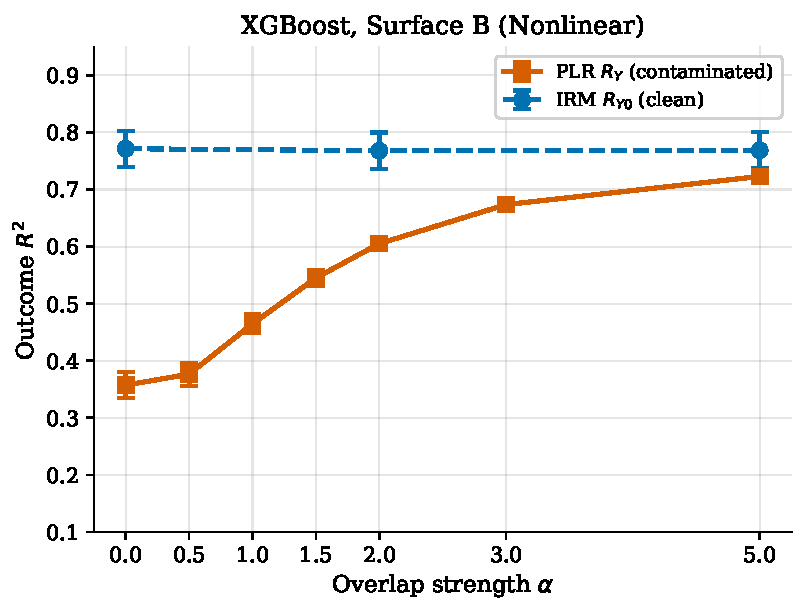
\includegraphics[width=\textwidth]{fig4_irm_vs_plr.pdf}
  \caption{IRM removes contamination. PLR's $R_Y$ drifts upward with $\alpha$ while IRM's $R_{Y0}$ remains stable. XGBoost, nonlinear surface.}
  \label{fig:irm_vs_plr}
\end{figure}

We evaluate diagnostic quality formally using the AUC for predicting whether a given replication's 95\% CI covers the true ATE:

\begin{table}[h!]
\centering
\caption{AUC for predicting 95\% CI coverage failure. Higher AUC indicates better discrimination between reliable and unreliable estimates. PLR grid uses all three learners (Lasso, Lasso+Logistic, XGBoost) across 7 overlap strengths; PLR (classifier learners) excludes Lasso to match IRM's classifier-only learner set, evaluated on the shared 3-overlap grid (0, 2, 5). Within-IRM improvements are statistically significant (paired bootstrap $p < 0.001$).}
\label{tab:auc}
\resizebox{\textwidth}{!}{%
\begin{tabular}{lcc}
\toprule
\textbf{Predictors} & \textbf{PLR AUC (Lin / Nonlin)} & \textbf{IRM AUC (Lin / Nonlin)} \\
\midrule
$R_D$ alone                                          & 0.566 / 0.649 & 0.797 / 0.747 \\
$R_D$ + outcome $R^2$                                & 0.564 / 0.645 & 0.822 / 0.776 \\
$R_D$ + outcome $R^2$ (classifier learners only)$^*$ & 0.793 / 0.763 & 0.822 / 0.776 \\
$R_D$ + local $R^2$ (both arms)                      & N/A\phantom{/ 0.000} & 0.838 / 0.795 \\
\midrule
\multicolumn{3}{l}{\footnotesize $^*$PLR restricted to Lasso+Logistic and XGBoost on shared 3-overlap grid ($\alpha \in \{0,2,5\}$); IRM uses all four learners on same grid.}
\bottomrule
\end{tabular}%
}
\end{table}

Under PLR, adding $R_Y$ to $R_D$ provides essentially no improvement (AUC 0.564 vs.\ 0.566), confirming that PLR's contaminated outcome metric adds noise rather than signal. Under IRM, $R_{Y0}$ adds modest value beyond $R_D$, and local $R^2$ from both arms achieves the best discrimination (Figure~\ref{fig:staircase}).

\begin{figure}[htbp]
  \centering
  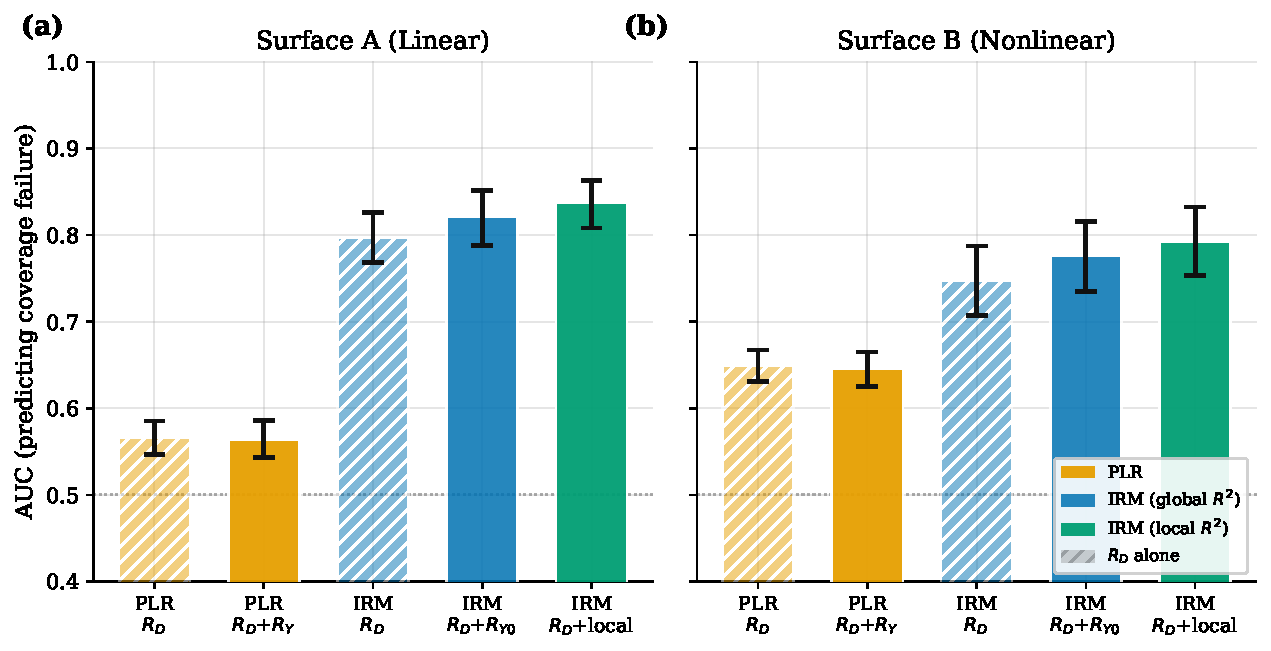
\includegraphics[width=\textwidth]{fig5_diagnostic_staircase.pdf}
  \caption{The diagnostic staircase. AUC comparison across PLR ($R_D + R_Y$), IRM global ($R_D + R_{Y0}$), and IRM local ($R_D + R_{Y0,\text{local}} + R_{Y1,\text{local}}$). Each within-IRM step is statistically significant ($p < 0.001$, paired bootstrap). The PLR--IRM gap reflects learner-composition differences in addition to framework differences; see Table~\ref{tab:auc} and Section~\ref{sec:results}.}
  \label{fig:staircase}
\end{figure}

\noindent\textbf{Decomposing the PLR--IRM gap.} The raw AUC gap (0.564 PLR vs.\ 0.822 IRM on the linear surface) is substantially a learner-composition artifact. Lasso fits propensity via linear regression rather than a classifier, producing anomalously high $R_D = 0.658$ at $\alpha = 5$ while simultaneously having poor coverage (27.0\%). This contradictory signal (high $R_D$ implying reliability, poor coverage contradicting it) suppresses PLR's diagnostic AUC. When Lasso is removed from PLR and the comparison is made on a shared three-overlap grid ($\alpha \in \{0,2,5\}$), PLR's AUC rises from 0.564 to 0.793. However, even this matched AUC is not practitioner-usable. Because PLR's $R_Y$ is contaminated, it rises as overlap weakens and coverage deteriorates: statistically, high $R_Y$ predicts failure rather than reliability. The AUC logistic classifier exploits this association automatically, treating high $R_Y$ as a warning signal. A practitioner interpreting $R_Y$ in the natural direction, reading high $R_Y$ as evidence of good outcome model fit, would reach the opposite conclusion and falsely increase confidence in an unreliable estimate. The residual IRM advantage shrinks to $+0.029$ on the linear surface and $+0.013$ on the nonlinear surface. The main benefit of IRM is therefore structural (it enforces classifiers for propensity by design and eliminates $R_Y$ contamination) rather than a large gain in diagnostic power over a well-specified PLR. Figure~\ref{fig:composition} visualises this decomposition.

\begin{figure}[htbp]
  \centering
  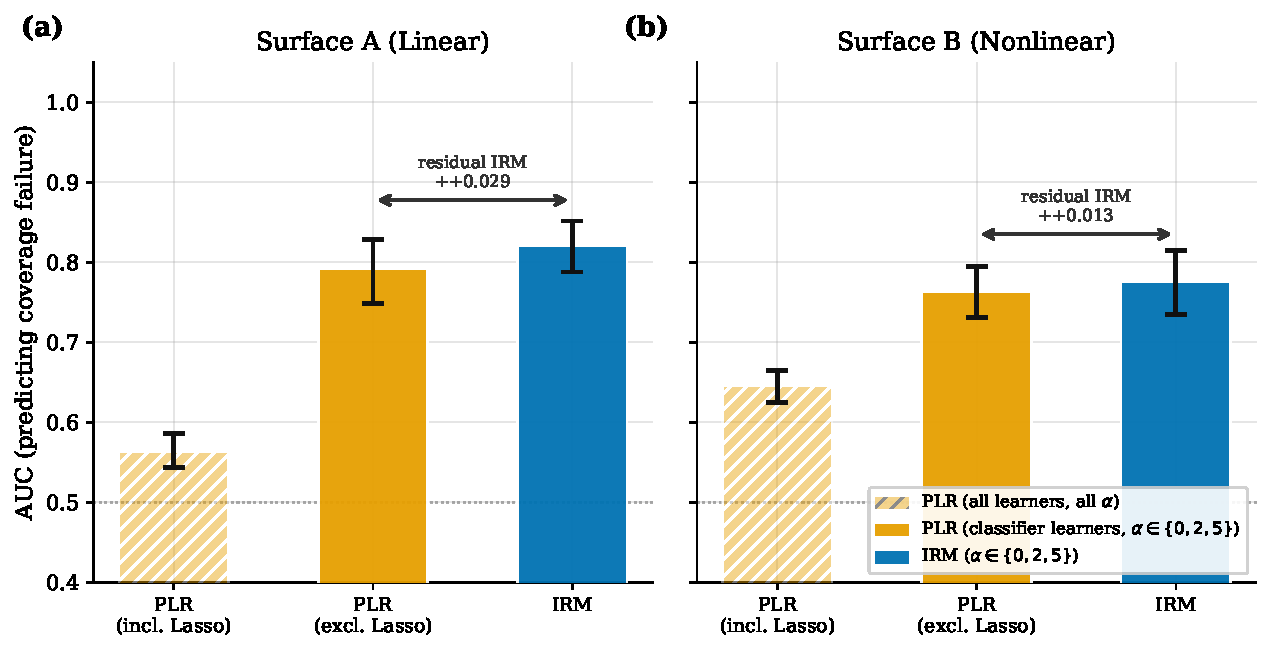
\includegraphics[width=\textwidth]{fig8_composition_decomposition.pdf}
  \caption{Decomposing the PLR--IRM AUC gap. The faded hatched bar shows PLR with all learners (including Lasso) across all overlap strengths; the solid bars restrict to the shared classifier learner set (Lasso+Logistic and XGBoost) and shared 3-overlap grid ($\alpha \in \{0, 2, 5\}$). The large jump from PLR (incl.\ Lasso) to PLR (excl.\ Lasso) reflects the learner-composition artifact: Lasso's anomalously high $R_D$ under misspecification suppresses discriminability. The bracket shows the residual IRM advantage after controlling for learner composition.}
  \label{fig:composition}
\end{figure}

\subsection{The Averaging Barrier and Local Diagnostics}

Global $R_{Y0}$ does not reliably rank learners by coverage. Ridge achieves the highest global $R_{Y0}$ (0.920) yet only 62\% coverage on the linear surface; XGBoost has lower $R_{Y0}$ (0.832) but 70\% coverage. The issue is that global $R^2$ averages over all units, masking fit failures in the thin-overlap extrapolation region where causal inference depends most heavily on the outcome model.

Restricting $R^2$ to controls with $\hat{m} > 0.5$ and treated with $\hat{m} < 0.5$ (the ``extrapolation region'') measures outcome fit precisely where it matters for causal inference. We compute local $R^2$ for both arms; the arm with weaker signal is naturally downweighted. The gap between global and local $R^2$ serves as a qualitative warning flag: Random Forest drops from 0.670 (global) to 0.519 (local), the largest gap ($= 0.15$) among all learners, and correspondingly shows the worst coverage (Figure~\ref{fig:averaging}). However, the gap alone does not add predictive power beyond local $R^2$ itself (gap-only AUC: 0.561 / 0.647).

\begin{figure}[htbp]
  \centering
  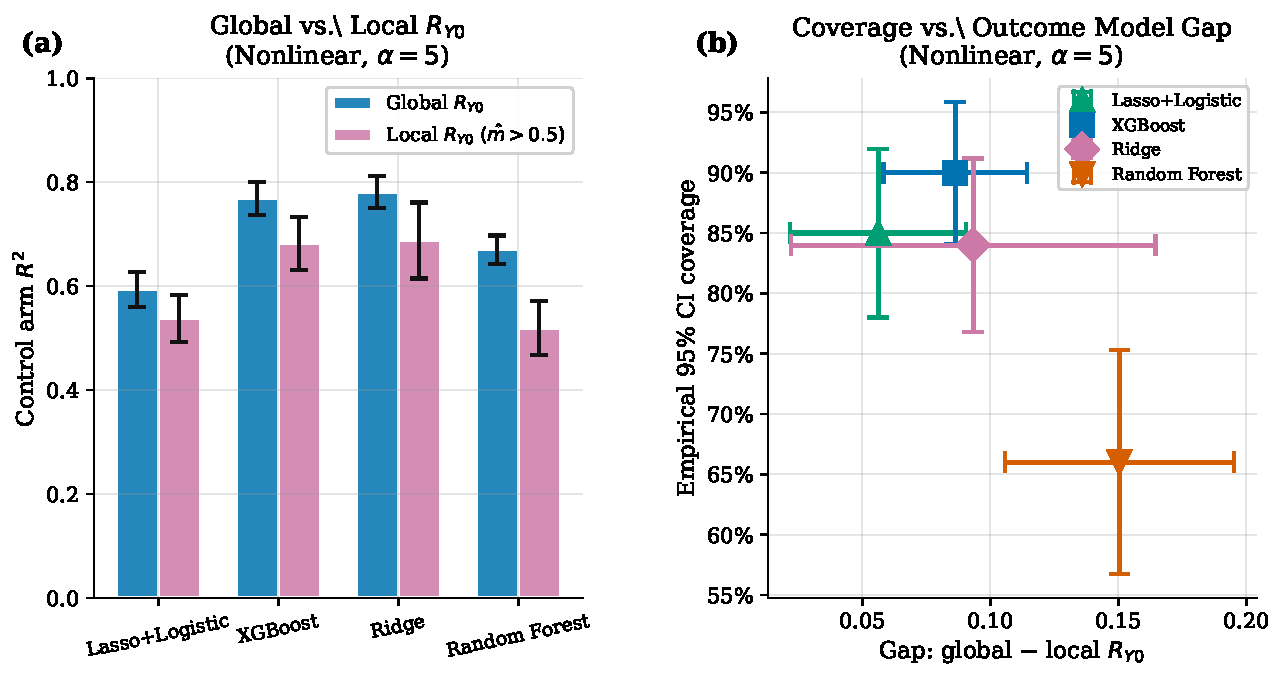
\includegraphics[width=\textwidth]{fig6_averaging_barrier.pdf}
  \caption{The averaging barrier. Left: global vs.\ local $R_{Y0}$ by learner under IRM, nonlinear surface, $\alpha = 5$. Right: gap (global minus local $R_{Y0}$) vs.\ coverage. Learners with larger gaps have worse coverage, suggesting outcome model failure in the extrapolation region.}
  \label{fig:averaging}
\end{figure}

\subsection{Robustness}

The inflation pattern for $R_D$ holds across all four propensity DGPs (structural, logistic, high-dimensional, threshold), three sample sizes ($n \in \{500, 985, 2000\}$), and with Random Forest as an alternative flexible learner. The contamination of PLR's $R_Y$ is a population-level structural property that does not diminish with sample size. IRM results are confirmed on a balanced grid of 2,400 estimations. The $\hat{m} > 0.5$ threshold for local $R^2$ is robust across sensitivity analyses using thresholds of 0.5, 0.7, and 0.8, as well as a top-$k = 30$ alternative.

\subsection{External Validation: LaLonde Covariates}
\label{sec:external_validation}

To check whether the diagnostic findings generalize beyond the IHDP covariate geometry, we replicate the IRM analysis on a semi-synthetic dataset built from the LaLonde employment training study \citep{LaLonde1986}. The LaLonde covariates (age, education, race, marital status, and earnings in 1974 and 1975; $n = 614$) differ substantially from IHDP's neonatal clinical measurements in domain, scale, and likely overlap structure. Treatment and outcomes are generated synthetically with a known ATE of 4.0, using the same structural propensity model as the primary simulation. Coverage is therefore measurable exactly.

We run both PLR and IRM with three learners (Ridge, Lasso+Logistic, Random Forest) across three overlap strengths ($\alpha \in \{0, 2, 4\}$) and two outcome surfaces (linear and localized nonlinear), with 20 replications per cell (360 estimations per framework). Table~\ref{tab:lalonde_auc} reports AUC for predicting coverage failure.

\begin{table}[h!]
\centering
\caption{External validation AUC on LaLonde covariates (360 estimations per framework). Each AUC is computed over all cells pooled within a surface.}
\label{tab:lalonde_auc}
\begin{tabular}{lcc}
\toprule
\textbf{Predictors} & \textbf{Linear AUC} & \textbf{Nonlinear AUC} \\
\midrule
PLR: $R_D$ + $R_Y$                                 & 0.701 & 0.798 \\
\midrule
IRM: $R_D$ alone                                   & 0.676 & 0.679 \\
IRM: $R_D$ + global $R_{Y0} / R_{Y1}$              & 0.859 & 0.701 \\
IRM: $R_D$ + local $R_{Y0} / R_{Y1}$ ($\hat{m}>0.5$) & 0.809 & 0.591 \\
\bottomrule
\end{tabular}
\end{table}

Three findings emerge. First, IRM global $R_{Y0}/R_{Y1}$ is the most reliable diagnostic: it adds substantial value over $R_D$ alone on the linear surface ($+0.183$ AUC) and remains interpretable throughout. Second, local $R_{Y0}/R_{Y1}$ does \emph{not} improve upon global on either surface; it is substantially worse on the nonlinear surface (0.591 vs.\ 0.701). LaLonde has 30\% baseline treatment probability, so the $\hat{m}>0.5$ threshold leaves fewer than 40 control units in the local region on average; local $R^2$ is estimated on too few units to be reliable. The failure mode is diffuse rather than concentrated, and global $R_Y$ already captures it. The local diagnostic improvement observed on IHDP does not replicate here.

Third, PLR $R_Y$ appears competitive on the nonlinear surface (AUC 0.798) but this is an artifact of contamination. Empirically, PLR $R_Y$ is positively correlated with overlap strength on the nonlinear surface ($r = +0.758$ with $\alpha$) while coverage falls, the anti-conservative signature of contamination. The logistic regression exploits this inverted signal (high $R_Y \to$ failure), but a practitioner interpreting $R_Y$ in the natural direction (high $= $ good fit) would draw the opposite conclusion. On the linear surface, PLR $R_Y$ actually moves in the correct direction ($r = -0.493$) but is redundant with $R_D$, which already captures the overlap signal. IRM dominates PLR on 3 of 4 surface--dataset combinations; the apparent exception is contamination-driven, not genuine diagnostic superiority.

% ===========================================================
% SECTION 6: DISCUSSION
% ===========================================================
\section{Discussion}

Our central finding is a fundamental tension between estimation robustness and diagnostic observability in DML. The orthogonalization that makes PLR robust to nuisance model errors simultaneously makes it impossible to build informative outcome-side diagnostics, because PLR's outcome model target $\mathbb{E}[Y \mid X] = g_0(X) + \tau \cdot m_0(X)$ conflates genuine outcome quality with treatment predictability. As overlap weakens, the treatment-prediction component becomes more learnable, artificially inflating $R_Y$ even as causal inference quality deteriorates. Switching to IRM resolves this structural contamination by estimating arm-specific outcome functions that are orthogonal to the treatment channel.

The practical implication for applied work is clear. When diagnostic observability matters (as it should whenever overlap is uncertain), practitioners should prefer IRM over PLR or run IRM alongside PLR as a reliability check. Under IRM, we recommend computing $R_D$ (propensity quality and overlap strength) alongside global arm-specific $R_{Y0}$ and $R_{Y1}$ (outcome fit for each arm). These diagnostics achieve AUC of 0.822 on IHDP (rising to 0.838 when local $R^2$ is additionally computed) and remain reliable on LaLonde. Practitioners can additionally compute local $R^2$ restricted to units in the extrapolation region ($\hat{m}>0.5$ for controls, $\hat{m}<0.5$ for treated). Importantly, the decision of whether to rely on local over global $R^2$ is itself data-driven and requires no knowledge of the true DGP. We recommend a two-step check. First, count $n_{\text{local}}$, the number of units in the local region; if this falls below a few dozen, local $R^2$ estimates are too noisy to trust and global $R_Y$ should be used. Second, if $n_{\text{local}}$ is adequate, examine the global--local gap: a large gap (global $R^2 \gg$ local $R^2$) indicates the outcome model extrapolates poorly in the extrapolation region, signaling concentrated failure and validating local $R^2$ as a sharper diagnostic. A small gap indicates failure is diffuse and global $R_Y$ already captures the relevant signal. These two checks reproduce the pattern across our datasets: on IHDP ($n_{\text{local}} \approx 150$ treated, large global--local gap at high $\alpha$), local provides further discrimination (AUC 0.838 vs.\ 0.822); on LaLonde ($n_{\text{local}} < 40$ controls, small gap from diffuse failure), local offers no additional value. The raw PLR baseline (0.56--0.65 on IHDP) understates PLR's true diagnostic potential: when PLR uses classifier-compatible learners on the same three-overlap grid, its AUC rises to 0.793, and the residual IRM advantage is modest (+0.029 on the linear surface). However, PLR $R_Y$ remains unreliable as a practitioner-facing diagnostic: on nonlinear surfaces it moves anti-conservatively (rising as coverage falls), so a high PLR $R_Y$ signals danger rather than reliability, the opposite of the natural interpretation. The gain from IRM is therefore structural and interpretive, not merely a modest improvement in discriminability. In all cases the diagnostics are continuous signals rather than binary flags and cannot guarantee that every coverage failure will be detected. Formal threshold rules for flagging unreliable estimates remain a direction for future work.

\medskip
\noindent\textbf{Relationship to existing diagnostics.} Our propensity-side diagnostic $R_D$ is the DML-native analog of several existing overlap diagnostics. \citet{Crump2009} trimming rules change the estimand by discarding units with extreme propensity scores, whereas $R_D$ measures residual treatment variation as a continuous signal without altering the estimand or requiring a separate analysis step. The effective sample size (ESS $= (\sum w_i)^2 / \sum w_i^2$) from the IPW literature captures similar intuition about observation concentration but requires explicit propensity weights. Recent work by \citet{Chernozhukov2025} proposes a condition number $\kappa_{\text{DML}} = 1/|\hat{J}_\theta|$ that is closely related to $1/\mathrm{Var}(\tilde{D})$, but does not separately assess outcome model quality. On the outcome side, \citet{Knaus2022} and \citet{Babino2020} each note the absence of adequate diagnostics for the cross-fitting stage; our contribution is to show both \emph{why} PLR's outcome metrics are structurally contaminated and \emph{how} IRM's arm-specific local diagnostics address the gap.

\medskip
\noindent\textbf{Limitations.} The primary simulation uses IHDP covariates as its base distribution. The external validation on LaLonde covariates supports the core findings ($R_D$ as a reliable overlap diagnostic, PLR $R_Y$ contamination, and IRM global $R_Y$ as an interpretable outcome diagnostic) but does \emph{not} replicate the local $R_Y$ improvement. The local diagnostic advantage on IHDP appears conditional on sufficient units in the extrapolation region and a concentrated failure mode. IHDP's 38\% treatment rate and $n=985$ yield roughly 150 treated units in the local region, enough for stable $R^2$ estimation; LaLonde's 30\% treatment rate and $n=614$ leave fewer than 40 control units in the local region, producing noisy estimates. Both conditions (adequate $n_{\text{local}}$ and a large global--local gap) are directly observable from the fitted propensity model and outcome residuals, so practitioners can assess local $R^2$ reliability without knowledge of the true DGP. The generality of the local refinement to other covariate geometries remains an open question. XGBoost hyperparameters are fixed rather than tuned. The PLR and IRM grids differ in learner composition (PLR includes Lasso as a propensity regressor; IRM uses classifiers only), which accounts for most of the raw AUC gap between frameworks; a fully matched comparison is available in Table~\ref{tab:auc} and discussed in Section~\ref{sec:results}.

% ===========================================================
% SECTION 7: CONCLUSION
% ===========================================================
\section{Conclusion}

This paper examines a previously underappreciated cost of DML's orthogonalization: the same mechanism that insulates treatment-effect estimates from nuisance model errors also degrades a practitioner's ability to assess whether those errors are severe enough to matter. Under PLR, the standard outcome-side diagnostic $R_Y$ is structurally contaminated by treatment predictability and moves anti-conservatively under overlap violation, providing no reliable warning signal; on nonlinear surfaces it can actively mislead practitioners by rising as coverage falls. Under IRM, this contamination disappears, and arm-specific global $R^2$ metrics provide interpretable, reliable diagnostic signal, with AUC reaching 0.822 on IHDP. Restricting $R^2$ to the extrapolation region (local $R^2$) provides a further improvement on IHDP (AUC 0.838) but does not generalize to LaLonde, where the lower treatment rate leaves too few units in the extrapolation region and the failure mode is diffuse across the support.

These findings have two direct implications for applied practice. First, we recommend computing IRM alongside any PLR analysis as a cheap reliability check, using $R_D$ and global arm-specific $R_{Y0}$, $R_{Y1}$ as the primary diagnostic signals. Local $R^2$ is a valuable refinement, and the decision to use it is itself data-driven: count $n_{\text{local}}$ units in the extrapolation region, then if sufficient, inspect the global--local gap. A large gap signals concentrated failure and validates local $R^2$ as a sharper diagnostic; a small gap indicates diffuse failure and global $R_Y$ already captures the relevant signal. Second, diagnostic observability deserves consideration as a first-class criterion when choosing between DML frameworks, alongside estimation efficiency and model flexibility. The ability to detect that a method is failing is as important as the method's theoretical properties when it succeeds. More broadly, this work highlights that robustness properties and self-diagnostic properties of estimators can be in fundamental tension, a consideration that deserves more attention in the design of modern causal inference pipelines.

% ===========================================================
% ACKNOWLEDGEMENTS
% ===========================================================
\section*{Acknowledgments}

This work draws substantially on the simulation framework and methodological insights developed by Professor Jennifer Hill. The semi-synthetic benchmark design (overlaying synthetic treatment assignments and outcomes onto real IHDP covariates to study causal inference under lack of common support) follows the approach introduced in \citet{Hill2011} and \citet{Hill2012}. The response surfaces used in our data-generating processes are adapted directly from Hill's original specifications. The authors appreciate our consultation with Professor Jennifer Hill.

% ===========================================================
% REFERENCES
% ===========================================================
\newpage
\begin{thebibliography}{99}

\bibitem[Babino et al.(2020)]{Babino2020}
Babino, L., Rotnitzky, A., \& Robins, J. (2020).
Machine learning for causal inference: on the use of cross-fit estimators.
\textit{Epidemiology}, 31(5), 724--730.

\bibitem[Chernozhukov et al.(2018)]{Chernozhukov2018}
Chernozhukov, V., Chetverikov, D., Demirer, M., Duflo, E., Hansen, C., Newey, W., \& Robins, J. (2018).
Double/debiased machine learning for treatment and structural parameters.
\textit{The Econometrics Journal}, 21(1), C1--C68.

\bibitem[Chernozhukov et al.(2025)]{Chernozhukov2025}
Chernozhukov, V., Newey, W.~K., \& Singh, R. (2025).
Ill-conditioned orthogonal scores in double machine learning.
\textit{arXiv preprint arXiv:2512.07083}.

\bibitem[Crump et al.(2009)]{Crump2009}
Crump, R.~K., Hotz, V.~J., Imbens, G.~W., \& Mitnik, O.~A. (2009).
Dealing with limited overlap in estimation of average treatment effects.
\textit{Biometrika}, 96(1), 187--199.

\bibitem[D'Amour et al.(2021)]{DAmour2021}
D'Amour, A., Ding, P., Feller, A., Lei, L., \& Sekhon, J. (2021).
Overlap in observational studies with high-dimensional covariates.
\textit{Journal of Econometrics}, 221(2), 644--654.

\bibitem[Hill(2011)]{Hill2011}
Hill, J.~L. (2011).
Bayesian nonparametric modeling for causal inference.
\textit{Journal of Computational and Graphical Statistics}, 20(1), 217--240.

\bibitem[Hill(2012)]{Hill2012}
Hill, J.~L. (2012).
Assessing lack of common support in causal inference using Bayesian nonparametrics: implications for evaluating the effect of breastfeeding on children's cognitive outcomes.
\textit{The Annals of Applied Statistics}, 6(4), 1386--1420.

\bibitem[LaLonde(1986)]{LaLonde1986}
LaLonde, R.~J. (1986).
Evaluating the econometric evaluations of training programs with experimental data.
\textit{American Economic Review}, 76(4), 604--620.

\bibitem[Khan \& Tamer(2010)]{Khan2010}
Khan, S., \& Tamer, E. (2010).
Irregular identification, support conditions, and inverse weight estimation.
\textit{Econometrica}, 78(6), 2021--2042.

\bibitem[Knaus(2022)]{Knaus2022}
Knaus, M.~C. (2022).
Double machine learning-based programme evaluation under unconfoundedness.
\textit{The Econometrics Journal}, 25(3), 602--627.

\bibitem[Rosenbaum \& Rubin(1983)]{Rosenbaum1983}
Rosenbaum, P.~R., \& Rubin, D.~B. (1983).
The central role of the propensity score in observational studies for causal effects.
\textit{Biometrika}, 70(1), 41--55.

\end{thebibliography}

\end{document}
